\documentclass[a4paper]{article}

\usepackage[english]{babel}
\usepackage[utf8x]{inputenc}
\usepackage{amsmath}
\usepackage{graphicx}
\usepackage{caption}
\usepackage{subcaption}

\usepackage[colorinlistoftodos]{todonotes}
\usepackage[letterpaper, margin=1in]{geometry}
\title{Database Representation and Application Implementation}
\author{
  Akash Garg\\
  \texttt{130070060}
  \and
  Shubham Jadhav\\
  \texttt{130050011}
  \and 
  Leena Madhuri\\
  \texttt{130050078}
}

\begin{document}
\maketitle
\textbf{Project: Gotweet}
\vspace{1cm}
\section*{{\underline{Database Representation}}}

%\line(1,0){350}\\
The database consists of 7 main tables.These tables are Junta, Followers, Tweets, Comments, Messages, Likes and Retweets. A brief description of each of the table is given below:
\begin{description}
\item[Junta: ] This table stores information about the users who are registered with the application. It stores information like name, username, password, date of birth, followers, following, email-id etc.  
\item[Followers: ] This table stores a row, for each 'follow' relation, which contains the follower and person being followed. This is similar to the following relationship in twitter. This table can be used both ways, i.e. to find the followers of a person or to find the people the person is following.
\item[Tweets: ] This table stores the actual tweets. Since the final motive of the app is to create social networking site like twitter, for each tweet we store some information like who tweeted it, tweet time, number of retweets, number of likes etc.
\item[Comments: ] We have also provided the user with the facility of commenting on tweets. Comments are stored separately from tweets with foreign key reference to the tweet id. Comments also have commenting time and commenter, the username of the person who wrote the comment.
\item[Messages: ] Along with public tweets the user also gets the facility to send private messages to other users. These messages are stored in the table 'messages'. The attributes include the sender, receiver, time of sending, etc.
\item[Likes: ] People might wish to know who has liked their tweet and also to prevent one person from liking a tweet twice we explictly store the 'like' relation. This relation contains who has liked which tweet.
\item[Retweet: ] Since retweet signifies that the tweet is not original from the person thus we have stored the retweets separately. Also this prevents a person from retweeting twice. The attributes of retweet are tweet-id(references to main tweet table) and person id who retweeted it.
\end{description}
\pagebreak

The main entities that are present in the database are Junta, Tweet, Message and Comment. The ER diagram of the relation is given below:\\
\begin{figure}[h]
\pdfcompresslevel0
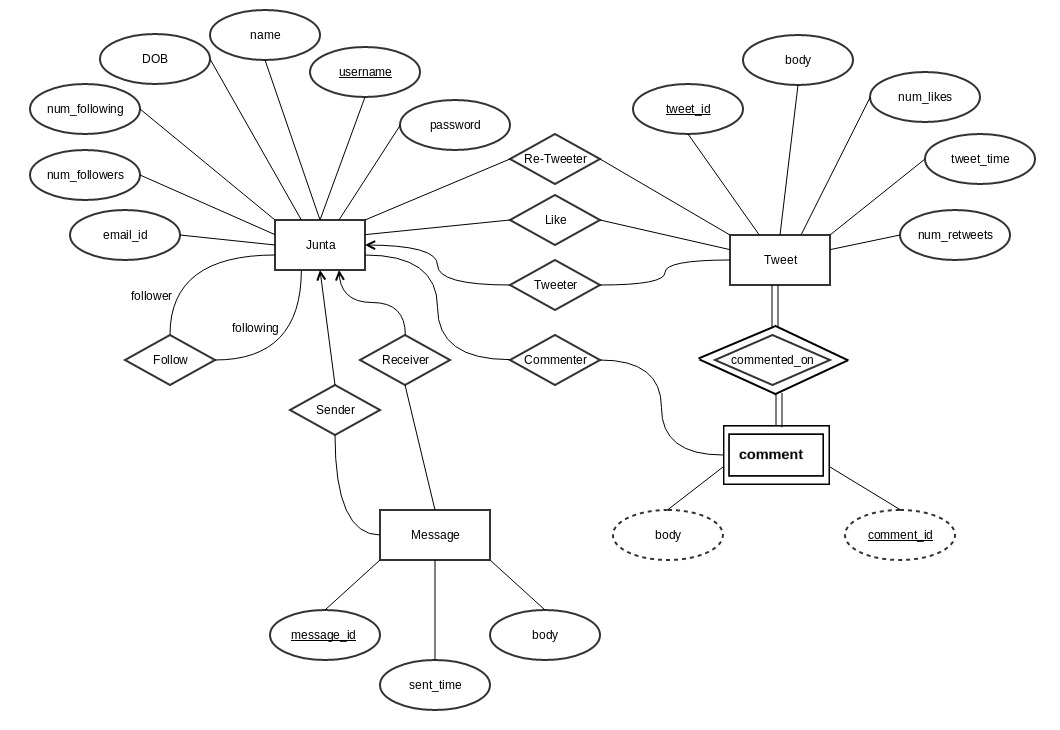
\includegraphics[width=18cm, height=14cm]{er2.jpg}
\caption{ER Diagram of the Database}
\end{figure}
\section*{{\underline{Normalization in Database Design}}}

We used normalization to eliminate data redundancy and undesirable characteristics. Normalization of the database served two main purpose:
\begin{itemize}
\item It eliminated data redundancy. We have reduced redundant data so that it can support large number of users.
\item Logical relations in data are preserved. Using various condition we preserved all the conditions that are required for consistency like only a valid user can comment on tweet, each tweet has a valid tweeter etc.
\end{itemize}

We started with 1-NF and went on to higher levels to remove all types of data redundancy and make tables which represent database well.

\section*{{\underline{Physical database design}}}
\vspace{1cm}
\subsection*{Database Consistency}
For a social networking application, database consistency is very important. There are various consistency requirements which have to be met. These include things like the username of commenter,liker,retweeter should be present in the junta table; the number of retweets, likes, comments should accurately represent actual number of comments. We have used various triggers for checking consistency, and all updates are done through functions. Thus the database is consistent all the time.

\subsection*{Tackling huge database problem}

\textbf{Problem} This is huge data centric application. The number of tweets, comments, likers could be very large. under these conditions it could be very difficult to retrive the tweets of a particular user from the table of all tweets. A user can also be following many users and to get tweets of each and every user from the tweets table would involve huge delays.
\textbf{Solution} This can be optimized easily. Since at one time we retrive tweets of a particular user so we store the tweets of one user on contagious location. We can also have b+ tree on users which can give the location on the tweets of user in the table. Thus the process of getting tweets is easier. The same could be applied for getting comments of a particular tweet and for other purposes. Also when we need tweets of more than one user we get tweets separately for each and then mix them.
\section*{{\underline{Implementation Details}}}
\vspace{1cm}
\subsection*{Classes}
We have classes in java corresponding to many table in the database including junta, followers, tweets, comments, messages, retweets etc. They have similar names. Thus it makes java functionality more easier. We can return tweets, person, comment etc. directly from any java function call.
\subsection*{{Functions}}
We have used the following main functions for retriving and updating data.
\begin{description}
\item[Gettweets: ]Takes as input the username of the person. Returns all the tweets the user is involved in. These may be either originally generated by the user, liked or retweeted.
\item[Getmessages: ]Takes input username. Returns a list of object message either sent or received by the user.
\item[Sendmessage: ]Takes the username of the sender and receiver and sends the message i.e. the message gets added to the database and the receiver can now see the message in his inbox.
\item[Getcomments: ]This function returns the comments for a particular tweet. This takes as input tweet-id.
\item[Searchpeople: ]It takes string as input and searches the junta(table of users) and returns the list of users with similar username. We have used special function to define this matching.
\item[Addtweet: ]Takes two entities as input, namely username who is posting the tweet and the message or the body of the tweet he/she is posting. It returns nothing since it will only add the pair to the database.
\item[Retweet/like: ]Void functions. The input values tweet\_id and username correspond to the user who retweeted/liked the tweet and makes appropriate changes to the database.
\item[Updateinfo: ]Takes the attributes to be changed and username and makes corresponding changes to the database.
\end{description}
\subsection*{{Servlets}}
The servlets provide the main user experience. They provide many sorts of data checks each specific to a page. We have many servlets and the perform all the checks on the data and calls the appropriate java functions for performing the changes as per the user instructions. Then they lend the people on the appropriate page as par the task done.

\begin{description}
\item[Login and Signup: ]This servlet implements the functionality for login and signup. When a user tries to signup it checks all the details are proper and the username has not been taken and adds the user to the list. The user than lands back on the homepage from where he can login. When user tries to login it checks whether the user is registered by checking the presence of username and password in junta table and if everything is correct the user lands on his homepage.%Implements the functions which are required to create an account and also does password verification while logging. The functions which it uses are updatepass and updatename. If signup is invoked, it returns to the login page. If login function is called, and the password is valid, then it goes to the homepage/NewsFeed of the user. Also calls the editing profile functions whose page is different but very similar to the signup page, except it won't have the username field.
\item[Tweet/Commenting: ]Has the functions which enables the user to tweet and comment on a particular tweet. Takes two entities as input, namely username who is posting and the tweet and the body he/she is posting. When called lands on the respective pages, where the change is visible. In case of comment it also takes the commentid as input.

\item[Liking/Retweeting: ]It takes the username and tweetid as input and performs the required task. This lands the user on the same page where he was before but now the changes are visible.

\item[Messaging: ]Implements the messaging functionality. Invokes the function getmessages when called. Takes input username. Returns a list of object message either sent or received by the user. After invoking, the user is able to see the message in the conversation form. Also performs the sendmessage functionality. When the user wishes to send a message, this is the servlet which respond to the request by calling the function Sendmessage.
\item[Search: ]Calls the searchpeople function and displays the list of people returned. This servlet respond to the search people requests of the user.


\end{description}

\section*{{User Interface}}
Currently we have designed all the pages in html and css. The servlets as described above provide movement and redirection between pages. We have tried to make the interface as simple as possible for new users. Some details as well as snapshots of the user interface are provided below:
\begin{itemize}
\item The user initially lands on the mainpage. There he can either choose to login or signup. Choosing the option lands him on another page where has has to fill his details accordingly and can signup/login. Only those users who have valid username and password can login.\\
\item Once the user has logged in. He lands on his homepage. Here he can see his tweets and tweets from people he is following. From here he can either go his own profile, search people, see people who he is following/who are following him, check messages or see details of a tweet.\\
\begin{figure}
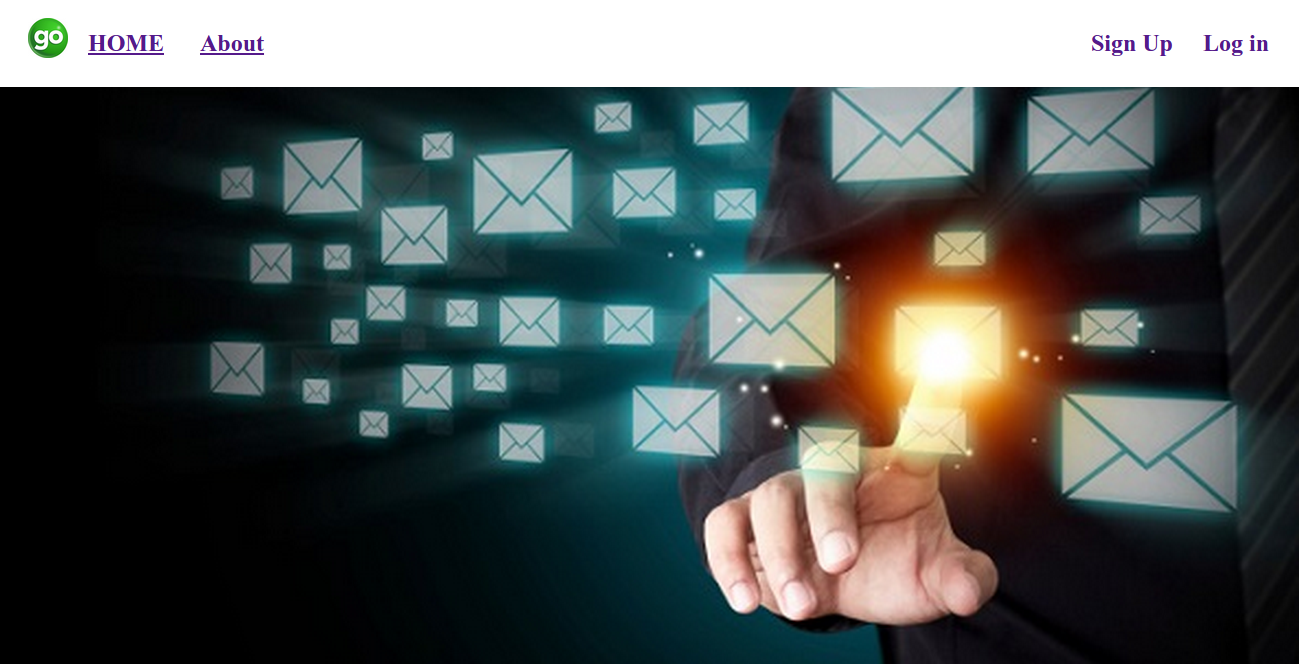
\includegraphics[width=15cm, height=10cm]{homepage.png}
\caption{Homepage}
\end{figure}
\begin{figure}
\centering
\begin{subfigure}{.5\textwidth}
  \centering
  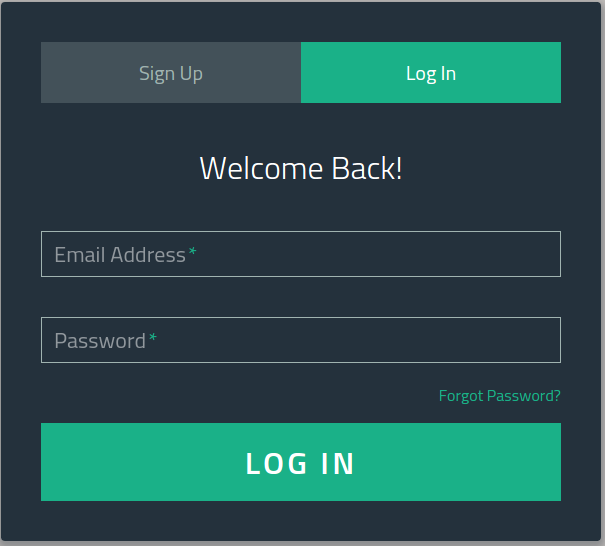
\includegraphics[width=5cm,height=5cm]{login_db.png}
  \caption{Login Page}
  \label{fig:sub1}
\end{subfigure}%
\begin{subfigure}{.5\textwidth}
  \centering
  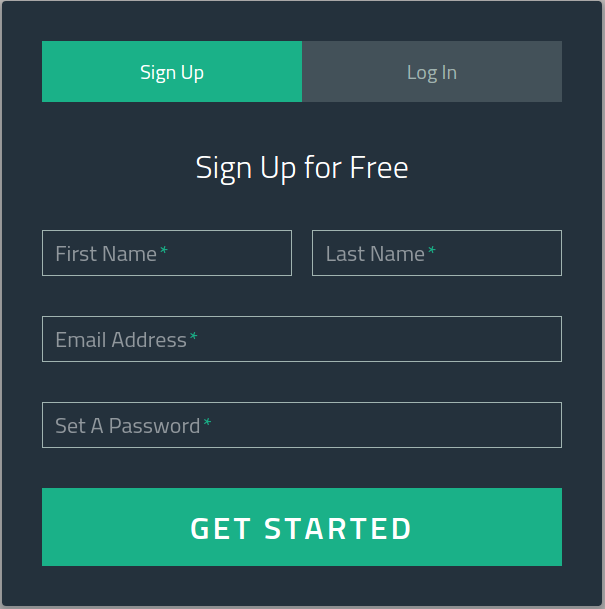
\includegraphics[width=5cm,height=5cm]{signup_dbproject.png}
  \caption{Signup Page}
  \label{fig:sub2}
\end{subfigure}
\caption{Login and Signup pages}
\label{fig:test}
\end{figure}
\item When a user visits his profile he can various details about himself and also has option to edit his details. He also see his tweets which he has tweeted, liked, commented on or retweeted.
\item When a user searches a person, he sees list of people in form of grid which have similar username. He can choose any user and visit his profile to see whether he is the one being searched. He also has the option to follow/unfollow the person.
\item When a user chooses to see the messages he sees a list of user he has communicated in the past. Clicking on any user gives the list of all the messages that have been exchanged amongst them. He can also send message to new user with whom he has not communicated yet just by providing his username and the message to be sent.
\item When a user wishes too see the people he is following or those who are following him, he can simply click the required option and the  list is shown to him in similar manner as when he searches for people.
\item When a user click a particular tweet, he can see the details of the tweet. This include all the comments that have been made of the tweet so far. Also he can comment on that tweet.
\end{itemize}
\section*{{\underline{Database Schema}}}

We have made the schema of the database. It has been presented below.\\
\begin{figure}[h]
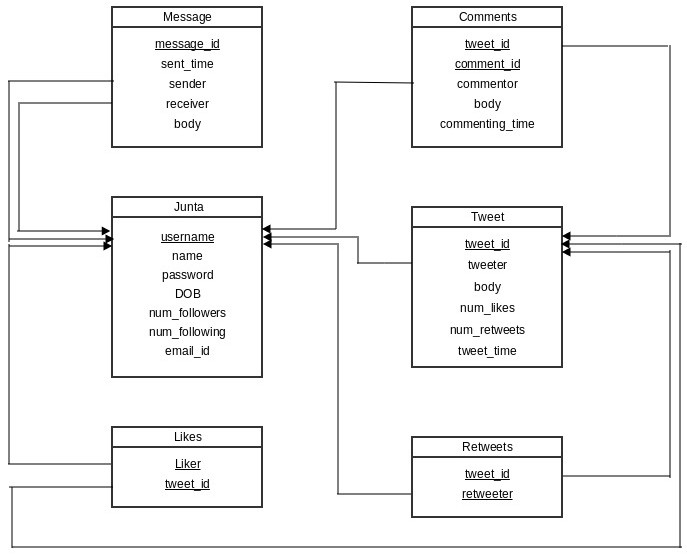
\includegraphics[width=15cm]{schema1.jpg}\\
\caption{The Schema of the Database}
\end{figure}
\begin{itemize}
\item The underlined entities represents the primary keys.
\item The arrows from one table to another shows foerign key relationship amongst tables on different attributes.
\end{itemize}

\end{document}


